\documentclass[11pt]{article}

% ---------------- Packages ----------------
\usepackage[margin=1in]{geometry}
\usepackage{amsmath,amssymb,amsthm}
\usepackage{graphicx}
\usepackage{hyperref}
\usepackage{fancyhdr}
\usepackage{enumitem}
\usepackage[UTF8]{ctex}
\usepackage{algorithm}
\usepackage{algpseudocode}
% ---------------- Header ----------------
\pagestyle{fancy}
\fancyhf{}
\lhead{Course Name}
\rhead{Homework \#1}
\cfoot{\thepage}

% ---------------- Title ----------------
\title{Homework 1}
\author{羊瑞 \\ 2300013091}
\date{\today}

% ---------------- Custom commands ----------------
\newcommand{\R}{\mathbb{R}}
\newcommand{\E}{\mathbb{E}}

% ---------------- Problem Environment ----------------
\newcounter{problem}

\newenvironment{problem}[1][]{
\stepcounter{problem}
\section*{Problem \theproblem\; #1}
}{}

\newenvironment{solution}{
\par\noindent\textbf{Solution.}\par\noindent
}{\qed}

\setlength{\parindent}{0pt}
% ---------------- Document ----------------
\begin{document}

\maketitle

\begin{problem} 
\begin{center}
    
\includegraphics[width=0.6\textwidth]{problems/10.1.png}
\end{center}
\end{problem}

\begin{solution}


设输入图 \(G=(V,E)\) 的顶点数为 \(n\)。

修改后的算法每次取一条尚未覆盖的边，只把这条边的一个端点加入顶点覆盖集。
设该算法在实例 \(I\) 上输出的顶点覆盖大小为 \(A(I)\)，最优解大小为 \(OPT(I)\)。

显然，任意顶点覆盖的大小至多为 \(n-1\)。因为只要取除某一个顶点外的所有顶点，就一定可以覆盖图中的所有边。因此有

\[
A(I)\leq n-1.
\]

同时，对于任意有边的图，

\[
OPT(I)\geq 1.
\]

所以该算法的近似比满足

\[
\frac{A(I)}{OPT(I)}\leq n-1.
\]

因此

\[
r\leq n-1.
\]

下面给出一个紧实例，说明该上界可以达到。

令

\[
G=\langle V,E\rangle,
\]

其中

\[
V=\{1,2,\ldots,n\},
\]

\[
E=\{(i,n)\mid 1\leq i\leq n-1\}.
\]

也就是说，\(G\) 是一个以顶点 \(n\) 为中心的星形图。

显然，只选择中心顶点 \(n\) 就可以覆盖所有边，因此

\[
OPT(I)=1.
\]

但是，修改后的算法可能依次选择边

\[
(1,n),(2,n),\ldots,(n-1,n),
\]

并且每次都只把叶子顶点加入顶点覆盖集。于是算法最终选择

\[
\{1,2,\ldots,n-1\}.
\]

因此

\[
A(I)=n-1.
\]

于是有

\[
\frac{A(I)}{OPT(I)}
=
\frac{n-1}{1}
=
n-1.
\]

所以该算法的最坏情况近似比为

\[
\boxed{r=n-1}.
\]

这说明，修改后的算法不再是常数近似算法，原来的 \(2\)-近似保证被破坏。
\end{solution}

\begin{problem}
\begin{center}
    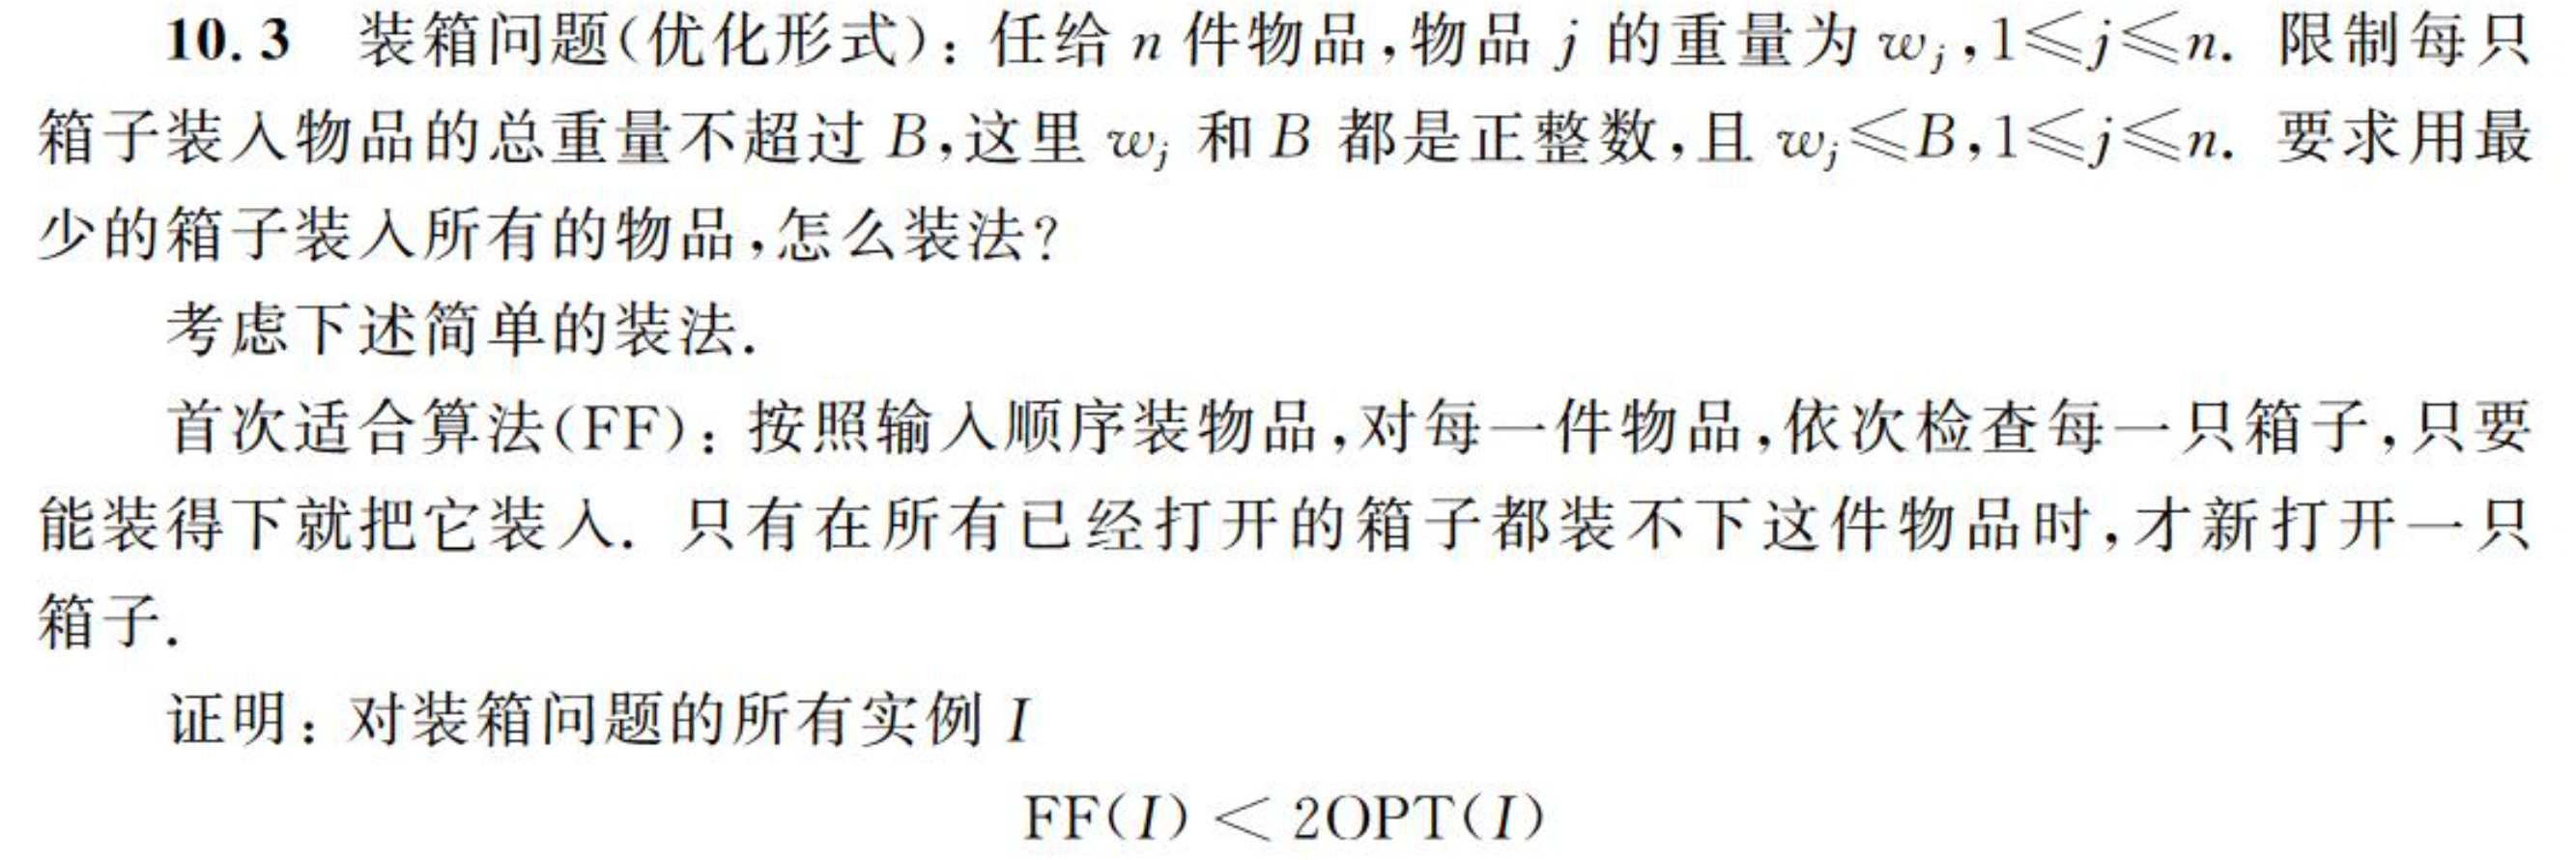
\includegraphics[width=0.6\textwidth]{problems/10.3.png}
\end{center}
\end{problem}

\begin{solution}

设实例 \(I\) 中每只箱子的容量为 \(B\)，首次适合算法最终使用了

\[
FF(I)=q
\]

只箱子，记这 \(q\) 只箱子的装载量分别为

\[
s_1,s_2,\ldots,s_q.
\]

下面证明一个关键性质：

\[
\forall\, 1\leq i<j\leq q,\qquad s_i+s_j>B.
\]

事实上，考虑第 \(j\) 只箱子被打开时放入的第一件物品，设其重量为 \(w\)。
由于首次适合算法只有在该物品无法放入前面所有已经打开的箱子时，才会打开第 \(j\) 只箱子，所以对于任意

\[
i<j,
\]

在当时第 \(i\) 只箱子的已有装载量 \(s_i'\) 满足

\[
s_i'+w>B.
\]

而最终第 \(i\) 只箱子的装载量满足

\[
s_i\geq s_i',
\]

第 \(j\) 只箱子的最终装载量满足

\[
s_j\geq w.
\]

因此

\[
s_i+s_j\geq s_i'+w>B.
\]

所以任意两只不同箱子的装载量之和都大于 \(B\)。

下面利用该性质分析近似比。

\[
情形一： q \text{ 为偶数。}
\]

把这 \(q\) 只箱子两两配对：

\[
(s_1,s_2),(s_3,s_4),\ldots,(s_{q-1},s_q).
\]

由上面的性质，每一对的装载量之和都大于 \(B\)，所以所有物品的总重量 \(W\) 满足

\[
W
=
\sum_{i=1}^q s_i
>
\frac{q}{2}B.
\]

另一方面，最优算法使用 \(OPT(I)\) 只箱子，每只箱子的容量为 \(B\)，所以

\[
W\leq OPT(I)\cdot B.
\]

因此

\[
\frac{q}{2}B<W\leq OPT(I)\cdot B.
\]

两边除以 \(B\)，得

\[
\frac{q}{2}<OPT(I),
\]

即

\[
q<2OPT(I).
\]

因为 \(q=FF(I)\)，所以

\[
FF(I)<2OPT(I).
\]

\[
\textbf{情形二：} q \text{ 为奇数。}
\]

此时把前 \(q-1\) 只箱子两两配对：

\[
(s_1,s_2),(s_3,s_4),\ldots,(s_{q-2},s_{q-1}).
\]

每一对的装载量之和都大于 \(B\)，因此

\[
W>\frac{q-1}{2}B.
\]

又因为

\[
W\leq OPT(I)\cdot B,
\]

所以

\[
\frac{q-1}{2}B<OPT(I)\cdot B.
\]

于是

\[
q-1<2OPT(I).
\]

由于 \(q\) 是奇数，而 \(2OPT(I)\) 是偶数，所以由

\[
q-1<2OPT(I)
\]

可知

\[
q<2OPT(I).
\]

因此仍有

\[
FF(I)<2OPT(I).
\]

综上，对于任意装箱问题实例 \(I\)，首次适合算法满足

\[
\boxed{FF(I)<2OPT(I)}.
\]
\end{solution}

\begin{problem}
\begin{center}
    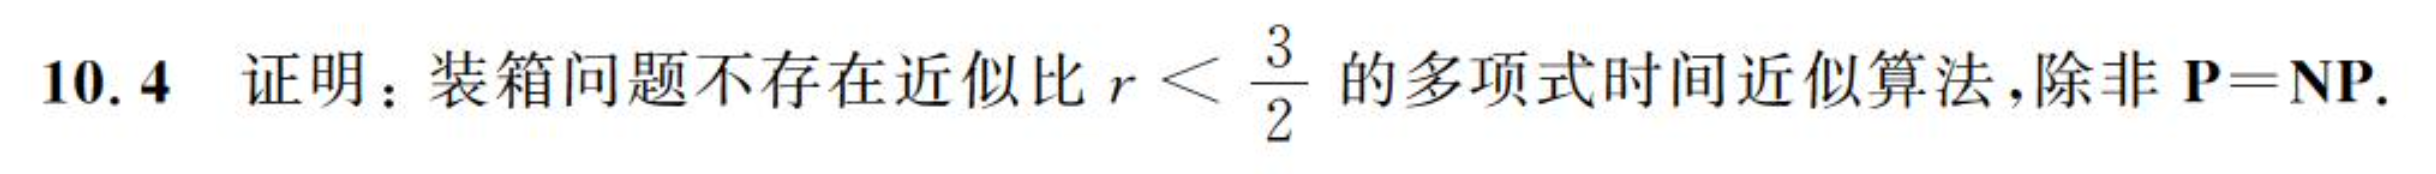
\includegraphics[width=0.6\textwidth]{problems/10.4.png}
\end{center}
\end{problem}

\begin{solution}

用反证法。假设存在一个多项式时间近似算法 \(A\)，其近似比满足

\[
r<\frac32.
\]

我们将利用算法 \(A\) 来多项式时间求解 \(\text{PARTITION}\) 问题。

\[
PARTITION 问题：
\]
给定正整数集合

\[
S=\{a_1,a_2,\ldots,a_n\},
\]

且

\[
\sum_{i=1}^n a_i = 2B,
\]

问是否存在一个子集 \(S'\subseteq S\)，使得

\[
\sum_{a_i\in S'} a_i = B.
\]

由该 \(\text{PARTITION}\) 实例构造一个装箱问题实例：

\[
\text{箱子容量为 } B,
\]

并且对每个整数 \(a_i\)，构造一件重量为 \(a_i\) 的物品。

下面分析该装箱实例。

如果原 \(\text{PARTITION}\) 实例有解，则存在一个子集的和为 \(B\)，另一个子集的和也为 \(B\)。因此所有物品可以恰好装入两个箱子中，所以

\[
OPT(I)=2.
\]

此时近似算法 \(A\) 输出的箱子数满足

\[
A(I)\leq r\cdot OPT(I)=2r.
\]

由于

\[
r<\frac32,
\]

所以

\[
2r<3.
\]

又因为 \(A(I)\) 是整数，所以

\[
A(I)\leq 2.
\]

而所有物品总重量为 \(2B\)，每只箱子容量为 \(B\)，所以至少需要两个箱子。因此

\[
A(I)=2.
\]

反过来，如果算法 \(A\) 输出

\[
A(I)=2,
\]

则说明这些物品可以装入两个容量为 \(B\) 的箱子中。由于所有物品总重量为

\[
2B,
\]

所以两个箱子都必须恰好装满，因而其中一个箱子中的物品重量和正好为

\[
B.
\]

这就给出了原 \(\text{PARTITION}\) 实例的一个解。

因此有

\[
\text{PARTITION 有解}
\iff
A(I)=2.
\]

也就是说，如果存在近似比

\[
r<\frac32
\]

的多项式时间装箱近似算法，则可以用它在多项式时间内判定 \(\text{PARTITION}\) 问题。

由于 \(\text{PARTITION}\) 是 NP 完全问题，所以这将推出

\[
P=NP.
\]

因此，除非

\[
P=NP,
\]

否则装箱问题不存在近似比

\[
r<\frac32
\]

的多项式时间近似算法。


装箱问题不存在  
\[
r<\frac32
\]
的多项式时间近似算法，除非  P=NP.

\end{solution}

\begin{problem}
\begin{center}
    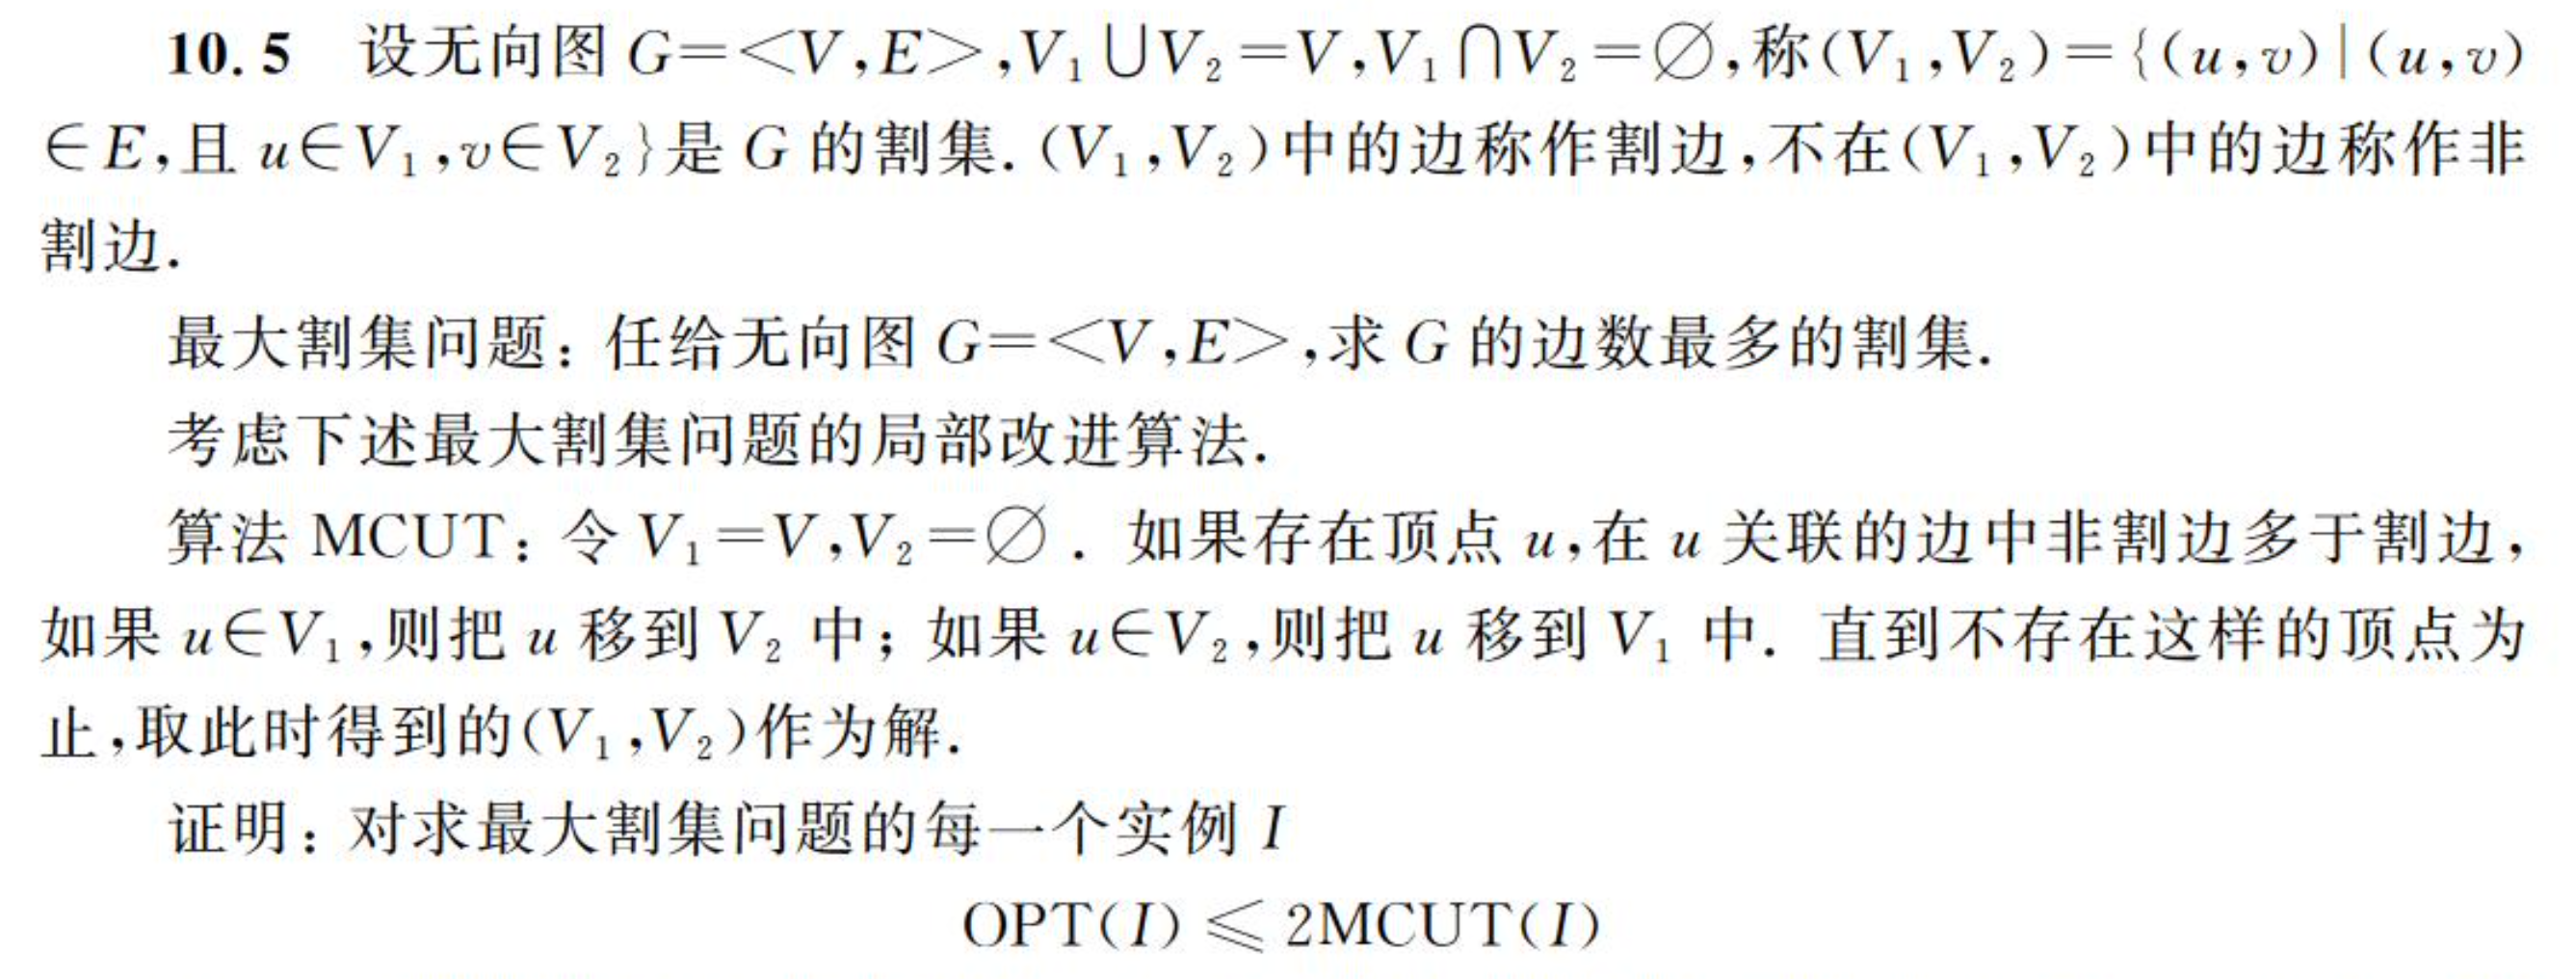
\includegraphics[width=0.6\textwidth]{problems/10.5.png}
\end{center}
\end{problem}

\begin{solution}


设算法最终得到的割为

\[
(V_1,V_2).
\]

记该割中的割边数为

\[
MCUT(I).
\]

对任意顶点 \(u\in V\)，记

\[
c(u)=\text{与 }u\text{ 关联的割边数},
\]

\[
\overline{c}(u)=\text{与 }u\text{ 关联的非割边数}.
\]

算法停止时，不存在这样的顶点 \(u\)：与 \(u\) 关联的非割边数多于割边数。也就是说，对任意

\[
u\in V,
\]

都有

\[
\overline{c}(u)\leq c(u).
\]

因此

\[
d(u)=c(u)+\overline{c}(u)\leq 2c(u),
\]

即

\[
c(u)\geq \frac{d(u)}{2}.
\]

对所有顶点求和，得

\[
\sum_{u\in V}c(u)
\geq
\frac12\sum_{u\in V}d(u).
\]

由握手定理可知

\[
\sum_{u\in V}d(u)=2|E|.
\]

另一方面，每条割边恰好被它的两个端点各计一次，所以

\[
\sum_{u\in V}c(u)=2MCUT(I).
\]

因此有

\[
2MCUT(I)
\geq
\frac12\cdot 2|E|
=
|E|.
\]

即

\[
MCUT(I)\geq \frac{|E|}{2}.
\]

而最大割的最优值显然不超过图中的总边数，即

\[
OPT(I)\leq |E|.
\]

于是

\[
OPT(I)
\leq
|E|
\leq
2MCUT(I).
\]

所以

\[
\boxed{OPT(I)\leq 2MCUT(I)}.
\]

因此该局部改进算法是一个 \(2\)-近似算法。
\end{solution}

\end{document}